\documentclass{beamer}

\usepackage[utf8]{inputenc}
\usepackage[english]{babel}
\usepackage{textpos}
\usepackage{graphicx}
\usepackage{textcomp}
\usepackage{animate}
\usepackage{comment}
%\usepackage{multicol}
%\setlength{\columnsep}{5cm}
\usepackage{amsmath}
\usepackage{amsfonts}
\usepackage{verbatim}
\usepackage{varwidth}
\usepackage{caption}
\usepackage{dcolumn}
\usepackage{amssymb}
\usepackage{algorithm}
\usepackage{algorithmic}
%\usepackage{physics}
\usepackage{hyperref}
\usepackage{scalerel,stackengine}
%\usepackage{fancyvrb}
\usepackage{enumitem}
\setlist[itemize]{label=\textbullet}
\usepackage{tikz}
\usepackage{pgfplots}

%\setbeamertemplate{itemize items}[circle]
%\setbeamertemplate{itemize subitem}[square]

\usefonttheme[onlymath]{serif}

\newcommand{\code}[1]{\texttt{#1}}
\newcommand{\shp}{$>>>$ }
\newcommand{\tab}{\hspace*{22pt}}

\usetheme{Madrid}

\title{Machine Learning with Scikit-Learn}
\author{EEC 3150}
\date{}

\institute{Trevecca Nazarene University}
 


%%%%%%%%% BEGIN DOCUMENT %%%%%%%%%
%%%%%%%%% BEGIN DOCUMENT %%%%%%%%%
%%%%%%%%% BEGIN DOCUMENT %%%%%%%%%

\begin{document}

% get title page 
\frame{\titlepage}
 
%%%%%%%%%%
%%%%%%%%%%
\begin{frame}	
	\frametitle{Outline}
	\tableofcontents	
\end{frame}


%%%%%%%%%%
%%%%%%%%%%
\section{Intro to ML}

\begin{frame}	
	\center{\Huge{Intro to ML}}
\end{frame}

\begin{frame}	
	\frametitle{Intro to ML}
	
	\begin{alertblock}{What is ML:}
		\footnotesize
		\textbf{Machine learning} is a field of data science/artificial intelligence which involves the use of statistical \textbf{models} to enable computers to learn and predict patterns in data
		\begin{itemize}
			\item A model is a function which can accurately map input data to output data \\
			$f($input$) = $ output
			\item Using a dataset of inputs/outputs to learn from, the model can learn the patterns (i.e., find a function $f$) and then, when given new input data, predict its output
		\end{itemize}
		
		\vspace{10pt}
		Example: create a model to predict real estate prices
		\begin{itemize}
			\item Input data: square footage, location, garage?, number of floors
			\item Output data: the price (a continuous value)
		\end{itemize}
		
		\vspace{10pt}
		Example: predict whether a patient has cancer
		\begin{itemize}
			\item Input data: age, gender, BMI, family history, environmental factors
			\item Output data: does/doesn't have cancer (a discrete label)
		\end{itemize}
	\end{alertblock}
\end{frame}

\begin{frame}	
	\frametitle{Intro to ML}
	
	\begin{block}{Some ML terms:}
		\scriptsize
		\begin{itemize}[itemindent=4.0em]
			\item[Dataset:] a collection of inputs/outputs
			\item[Samples:] entries in the dataset
			\item[] (rows in the dataset)
			\item[Features:] the input data (usually $X$, a 2D array $(N_{samp},N_{feat})$)
			\item[] (columns in the dataset)
			\item[Labels:] the output data (usually $y$, a 1D array $(N_{samp})$) \\
			\item[] (sometimes called ``target'')
			\item[] (a special column in the dataset)
			\item[Model:] a function $f$ which predicts labels based on features
			\item[Training:] the process by which the model ``learns'' the patterns in a dataset
			\item[Testing:] the process by which a model's performance/accuracy is evaluated
			\item[Loss function:] a function which evaluates the amount of error in the model
			\item[] (sometimes called error, must be minimized,
			\item[] training is minimizing the loss function)
		\end{itemize}
	\end{block}
	
\end{frame}

\begin{frame}	
	\frametitle{Intro to ML}
	
	\begin{block}{Types of ML:}
		\footnotesize
		\begin{itemize}%[itemindent=1em, align=left]
			\item Supervised learning: a type of learning where the dataset has features AND labels and the goal is to predict the labels based on the features 
			\begin{itemize}
				\item Regression (label is continuous)
				\item Classification (label is categorical/discrete)
			\end{itemize}
			\item Unsupervised learning: a type of learning where the dataset ONLY has features and the goal is to assign a set of reasonable labels
			\begin{itemize}
				\item Clustering
			\end{itemize}
			\item Generative learning: a type of learning where the goal is to create more data like the features
			\begin{itemize}
				\item AI chatbots
				\item AI image generators
			\end{itemize}
		\end{itemize}
	\end{block}
	
\end{frame}

\begin{frame}	
	\frametitle{Intro to ML}
	
	\begin{block}{Python libraries for ML:}
		\begin{itemize}%[itemindent=1em, align=left]
			\item Scikit-learn (we'll use this one) \\
			\url{https://scikit-learn.org/stable/modules/classes.html}
			\item Tensorflow, Keras, PyTorch (neural networks)
			\item XGBoost (gradient boosting)
		\end{itemize}
	\end{block}
	
\end{frame}


%%%%%%%%%%
%%%%%%%%%%
\section{Supervised Learning}
\subsection{Regression}

\begin{frame}	
	\center{\Huge{Supervised Learning: \\ Regression}}
\end{frame}

\begin{frame}
	\frametitle{Supervised Learning: Regression}
	
	\begin{alertblock}{Linear regression:}
%		\footnotesize
		\textbf{Linear regression} is the process of fitting a linear model to the data
		
		\vspace{20pt}
		Single regression: fitting one feature ($x$) to the label
		\begin{equation*}
			f(x) = a x + b
		\end{equation*}
		
		Multiple regression: fitting several features ($x,x'$) to the label
		\begin{equation*}
			f(x, x') = a x + b x' + c
		\end{equation*}
		
		\vspace{10pt}
		Goal: find the slopes/intercept which minimize the loss
	\end{alertblock}

\end{frame}

\begin{frame}
	\frametitle{Supervised Learning: Regression}
	
	\begin{block}{Linear regression:}
		\small
		
		Loss: sum of squared errors/residuals (SSE):
		\begin{align*}
			\textrm{loss} & = \sum_{i=0}^{N_{samp}-1} \Big( f(x_i) - y_i \Big)^2 \\
			\textrm{loss}(a,b) & = \sum_{i=0}^{N_{samp}-1} \Big( (a x_i + b) - y_i \Big)^2
		\end{align*}
		
		Minimize (ordinary least squares - OLS):
		\begin{equation*}
			\min_{a,b} \textrm{loss}(a,b)
		\end{equation*}
		
		Other loss functions:
		\begin{itemize}
			\item Mean-squared error (MSE = loss$/N_{samp}$)
			\item Root mean-squared error (RMSE = $\sqrt{\textrm{MSE}}$)
		\end{itemize}
	\end{block}

\end{frame}

\begin{frame}
	\frametitle{Supervised Learning: Regression}
	
	\begin{block}{Model evaluation:}
		There are several metrics for evaluating the quality of a linear regression model:
		\begin{itemize}
			\item Loss
			\item $R^2$ (square of Pearson correlation coefficient)
		\end{itemize}
	\end{block}

\end{frame}

\begin{frame}
	\frametitle{Supervised Learning: Regression}
	
	\begin{alertblock}{Linear regression:}
		\footnotesize
		
		\minipage{0.45\textwidth}
			Regression (or curve fitting) is the process of creating a model which uses features to predict continuous labels
			
			\vspace{10pt}
			Some example data: \\
			
			\begin{tabular}{|c|c|c|}
				\hline
				& Features & Labels \\
				\hline
				& Sq ft & Price \\
				\hline
				0 & 1,500 & 210,000 \\
				\hline
				1 & 2,000 & 280,000 \\
				\hline
				2 & 1,650 & 260,000 \\
				\hline
				3 & 2,200 & 320,000 \\
				\hline
			\end{tabular}
		\endminipage\hfill
		\minipage{0.02\textwidth}
		\endminipage\hfill
		\minipage{0.53\textwidth}
			Let
			\begin{itemize}
				\item $N_{samp}=4$ be the number of samples
				\item $N_{feat}=1$ be the number of features
				\item $X_{i,j}$ be $j$-th feature of the $i$-th sample \\
				Ex: $X_{2,0} = 1,650$
				\item $y_i$ be the $i$-th sample's label \\
				Ex: $y_{0} = 210,000$
				\item $f(\cdot)$ be our model
				\item loss: sum of squared errors (SSE)
			\end{itemize}
			
			\begin{equation*}
				\textrm{loss} = \sum_{i=0}^{N_{samp}-1} \Big( f(X_{i,0}) - y_i \Big)^2
			\end{equation*}
			
			\vspace{10pt}
			Goal: find the model $f$ which minimizes the loss
		\endminipage\hfill
	\end{alertblock}

\end{frame}

\begin{frame}
	\frametitle{Supervised Learning: Regression}
	
	\begin{alertblock}{Linear regression:}
		\footnotesize
		
		\minipage{0.45\textwidth}
			Regression (or curve fitting) is the process of creating a model which uses features to predict continuous labels
		
			\vspace{10pt}
			Goal: find the model $f$ which minimizes the loss
			
			\vspace{10pt}
			Some example data: \\
			
			\begin{tabular}{|c|c|c|c|}
				\hline
				& \multicolumn{2}{|c|}{Features} & Labels \\
				\hline
				& Sq ft & Floors & Price \\
				\hline
				0 & 1,500 & 1 & 210,000 \\
				\hline
				1 & 2,000 & 2 & 280,000 \\
				\hline
				2 & 1,650 & 1 & 260,000 \\
				\hline
				3 & 2,200 & 3 & 320,000 \\
				\hline
			\end{tabular}
		\endminipage\hfill
		\minipage{0.05\textwidth}
		\endminipage\hfill
		\minipage{0.5\textwidth}
			Let
			\begin{itemize}
				\item $N_{samp}=4$ be the number of samples
				\item $N_{feat}=2$ be the number of features
				\item $X_{i,j}$ be $j$-th feature of the $i$-th sample \\
				Ex: $X_{3,1} = 3$
				\item $y_i$ be the $i$-th sample's label \\
				Ex: $y_{0} = 210,000$
				\item $f(\cdot,\cdot)$ be our model
				\item loss: sum of squared errors (SSE)
			\end{itemize}
			
			\begin{equation*}
				\textrm{loss} = \sum_{i=0}^{N_{samp}-1} \Big( f(X_{i,0},X_{i,1}) - y_i \Big)^2
			\end{equation*}
		\endminipage\hfill
	\end{alertblock}

\end{frame}


\subsection{Classification}

\begin{frame}	
	\center{\Huge{Supervised Learning: \\ Classification}}
\end{frame}

\begin{frame}
	\frametitle{Supervised Learning: Classification}
	
	\begin{alertblock}{Classification:}
		\footnotesize
		
		\minipage{0.45\textwidth}
			Classification is the process of creating a model which uses features to predict discrete labels
			
			\vspace{5pt}
			Some example data: \\[-15pt]
			
			\begin{figure}[ht]
				\centering
				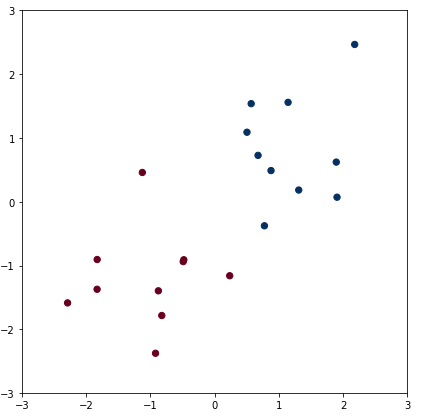
\includegraphics[width=\linewidth]{Classification_01}
			\end{figure}
		\endminipage\hfill
		\minipage{0.05\textwidth}
		\endminipage\hfill
		\minipage{0.5\textwidth}
			What we're given:
			\begin{itemize}
				\item 2 features (on the x,y axes)
				\item A discrete label, 2 classes: red and blue
			\end{itemize}
			The goal:
			\begin{itemize}
				\item Create a model which can predict the class for new data
			\end{itemize}
			Some thoughts:
			\begin{itemize}
				\item The reds and blues each tend to cluster together
				\item New data that is firmly within the red cluster can be confidently classified as red (same for blue)
				\item New data which appears somewhere in b/t the two clusters in less clear how to classify
			\end{itemize}
		\endminipage\hfill
	\end{alertblock}

\end{frame}

\begin{frame}
	\frametitle{Supervised Learning: Classification}
	
	\begin{block}{$k$ Nearest Neighbors Classification (KNN):}
		\footnotesize
		Method:
		\begin{itemize}
			\item When given a new data point, find its $k$ (an integer) nearest neighbors (the points closest to it)
			\item Assign the new point the label which is most frequent among its neighbors
			\item Choose the value of $k$ which gives the lowest loss/highest accuracy 
		\end{itemize}
		Loss function:
		\begin{itemize}
			\item There are many good loss functions for classification (cross entropy...)
			\item We will instead just maximize the accuracy (instead of minimizing loss)
		\end{itemize}
	\end{block}

\end{frame}

\begin{frame}
	\frametitle{Supervised Learning: Classification}
	
	\begin{block}{Train/test splitting:}
		\footnotesize
		Motivation:
		\begin{itemize}
			\item We train our model using only the data we have at our disposal, but when your model actually gets used by someone, it will see NEW data
			\item We want our model to generalize to new data (it needs to do more than just predict the data it was trained on)
			\item To solve this, we split our data into two parts:
			\begin{itemize}
				\item Training data: the data we use to create the model
				\item Testing data: the data was use to evaluate the model's performance
			\end{itemize}
			\item Once we find out what model parameters give the highest accuracy, we can then train on the whole dataset and let that be our final model
		\end{itemize}
		Some notes:
		\begin{itemize}
			\item Generally, we use an 80/20 split between training/test, respectively
			\item Generally, the training accuracy will be higher than the testing accuracy (makes sense since the model was designed with that data)
		\end{itemize}
	\end{block}

\end{frame}

\begin{frame}
	\frametitle{Supervised Learning: Classification}
	
	\begin{block}{Accuracy vs. precision/recall:}
		\begin{itemize}
			\item Sometimes accuracy is too simple of an evaluation metric
			\item We can also use precision and recall
			\item \url{https://towardsdatascience.com/accuracy-precision-recall-or-f1-331fb37c5cb9}
		\end{itemize}
	\end{block}

\end{frame}


\end{document}






